\chapter{Contador de programa (\texttt{prog\_cnt})}
\label{cap:prog_cnt}

\section{Especificação}

O \texttt{prog\_cnt} é um contador síncrono módulo 2048 (de 0 a 2047), com reset assíncrono e carga síncrona \cite{tp2}. Ele tem duas saídas: \texttt{pc\_out}, a saída dos \textit{flip-flops}, e \texttt{next\_pc\_out}, a entrada dos \textit{flip-flops}, ou seja, o valor que será carregado na próxima borda de subida (combinacional). A entrada \texttt{pc\_ctrl} escolhe a função, e todas são síncronas com \texttt{clk\_in} (Quadro~\ref{quad:pc-ctrl}). O reset assíncrono zera o contador e tem preferência sobre todas as outras entradas.

\begin{quadro}[htb]
  \caption{Funções do contador de programa, selecionadas por \texttt{pc\_ctrl}.}
  \label{quad:pc-ctrl}
  \centering
  \begin{tabular}{cl}
    \hline
    \texttt{pc\_ctrl} & Função \\ \hline
    \texttt{00} & Permanece como está \\
    \texttt{01} & Carrega o topo da pilha (entrada \texttt{from\_stack}) \\
    \texttt{10} & Carrega um novo valor (entrada \texttt{new\_pc\_in}) \\
    \texttt{11} & Incrementa o contador ($+1$) \\ \hline
  \end{tabular}
  \fonte{Adaptado de \textcite{tp2}.}
\end{quadro}

A Figura~\ref{fig:bloco-prog-cnt} mostra o diagrama de blocos e o Quadro~\ref{quad:portas-prog-cnt} descreve as portas. A ligação com a pilha, em que \texttt{from\_stack} vem de \texttt{stack\_out} e \texttt{pc\_out} vai para \texttt{stack\_in}, será feita no quarto trabalho, conforme a especificação.

\begin{figure}[htb]
\caption{Diagrama de blocos do contador de programa.}\label{fig:bloco-prog-cnt}
\centering
\begin{tikzpicture}[>={Stealth[length=2mm]}]
  \renewcommand{\fio}{1.0}
  \node[draw, minimum width=3.2cm, minimum height=4.4cm, font=\large\bfseries] (bloco) {prog\_cnt};
  \pentrada{1.8}{nrst}{}
  \pentrada{1.0}{clk\_in}{}
  \pentrada{0.2}{pc\_ctrl[1..0]}{line width=1.2pt}
  \pentrada{-0.6}{new\_pc\_in[10..0]}{line width=1.2pt}
  \pentrada{-1.4}{from\_stack[10..0]}{line width=1.2pt}
  \psaida{0.7}{next\_pc\_out[10..0]}{line width=1.2pt}
  \psaida{-0.7}{pc\_out[10..0]}{line width=1.2pt}
\end{tikzpicture}
\fonte{Elaborada pelos autores, com base em \textcite{tp2}.}
\end{figure}

\begin{quadro}[htb]
  \caption{Portas do contador de programa.}
  \label{quad:portas-prog-cnt}
  \centering
  \begin{tabular}{lcp{8.8cm}}
    \hline
    Porta & Direção & Descrição \\ \hline
    \texttt{nrst} & entrada & \textit{Reset} assíncrono, ativo em nível baixo; zera o contador \\
    \texttt{clk\_in} & entrada & Clock; incremento e carga acontecem na borda de subida \\
    \texttt{pc\_ctrl[1..0]} & entrada & Função do contador (Quadro~\ref{quad:pc-ctrl}) \\
    \texttt{new\_pc\_in[10..0]} & entrada & Valor carregado com \texttt{pc\_ctrl = "10"} \\
    \texttt{from\_stack[10..0]} & entrada & Valor carregado com \texttt{pc\_ctrl = "01"} \\
    \texttt{next\_pc\_out[10..0]} & saída & Próximo valor do contador (combinacional) \\
    \texttt{pc\_out[10..0]} & saída & Valor atual do contador (saída dos \textit{flip-flops}) \\ \hline
  \end{tabular}
  \fonte{Adaptado de \textcite{tp2}.}
\end{quadro}

\section{Implementação}

\subsection{Arquitetura}

O contador é descrito em duas partes, como no diagrama funcional da especificação (Figura~\ref{fig:rtl-prog-cnt}), com dois sinais internos: \texttt{pc}, a saída dos \textit{flip-flops}, e \texttt{next\_pc}, a entrada deles.

\begin{itemize}
  \item \textbf{Parte combinacional}: um \texttt{WITH}/\texttt{SELECT} sobre \texttt{pc\_ctrl} calcula \texttt{next\_pc}: \texttt{pc} (manter), \texttt{from\_stack}, \texttt{new\_pc\_in} ou \texttt{pc + 1}. Como \texttt{pc} tem 11 bits e o pacote \texttt{std\_logic\_unsigned} descarta o \textit{carry} final, a soma volta a 0 depois de 2047, o que é o módulo 2048 exigido.
  \item \textbf{Parte sequencial}: um \texttt{process} sensível a \texttt{nrst} e \texttt{clk\_in} zera \texttt{pc} com o reset e, na borda de subida, carrega \texttt{pc <= next\_pc}.
  \item As saídas \texttt{next\_pc\_out} e \texttt{pc\_out} são atribuições concorrentes dos dois sinais.
\end{itemize}

\subsection{Decisões de projeto}

\begin{itemize}
  \item \textbf{Código concorrente na parte combinacional}: a especificação recomenda dois \texttt{process}, um para cada parte. A parte combinacional foi escrita como um \texttt{WITH}/\texttt{SELECT}, que é equivalente e mais curto, e a lista de sensibilidade (que num processo combinacional é fonte de erros) deixa de existir. O resultado sintetizado é o mesmo da Figura~\ref{fig:rtl-prog-cnt}.
  \item \textbf{Alternativa \texttt{WHEN OTHERS}}: o \texttt{WITH}/\texttt{SELECT} precisa cobrir todos os valores do tipo de \texttt{pc\_ctrl}; os quatro valores binários têm ramo próprio e o \texttt{WHEN OTHERS} (mantém) cobre os demais, que só existem em simulação (como \texttt{'X'} ou \texttt{'U'}), sem custo de \textit{hardware}.
  \item \textbf{\texttt{next\_pc} como sinal}: guardar o próximo valor num sinal permite usá-lo tanto na saída \texttt{next\_pc\_out} quanto na entrada dos \textit{flip-flops} sem duplicar a lógica.
\end{itemize}

\subsection{Circuito em nível RTL}

A Figura~\ref{fig:rtl-prog-cnt} mostra a interpretação feita pelo RapidRTL: o registrador \texttt{pc} (\texttt{\$adff}, com reset assíncrono), um somador com a constante 1 e um multiplexador de quatro entradas (\texttt{pc}, \texttt{from\_stack}, \texttt{new\_pc\_in} e \texttt{pc + 1}) cujo seletor é derivado de \texttt{pc\_ctrl} por comparadores com as constantes \texttt{01}, \texttt{10} e \texttt{11}. A saída do multiplexador alimenta a entrada D do registrador e a saída \texttt{next\_pc\_out}, e a saída do registrador é \texttt{pc\_out} e a entrada do somador e do ramo ``manter''. O Quartus aloca 11 \textit{flip-flops} e 33 elementos lógicos.

\begin{figure}[htb]
  \centering
  \caption{Circuito do contador de programa em nível RTL.}
  \label{fig:rtl-prog-cnt}
  \includegraphics[width=0.6\textwidth, height=0.5\textheight, keepaspectratio]{prog_cnt_rtl.pdf}
  \fonte{Elaborado a partir do site RapidRTL, com base no arquivo \texttt{project/prog\_cnt/prog\_cnt.vhd}.}
\end{figure}

\subsection{Código-fonte}

O Código~\ref{lst:prog-cnt} apresenta a entidade e a arquitetura completas, com comentários.

\blocovhdl{Descrição VHDL do contador de programa.}{lst:prog-cnt}{prog_cnt}{prog_cnt.vhd}

\section{Simulação e resultados}

\subsection{Metodologia}

O projeto tem quatro formas de onda (arquivos \texttt{.vwf} em \texttt{project/prog\_cnt/}), todas com clock de 20\,ns e reset inicial:

\begin{itemize}
  \item \texttt{prog\_cnt.vwf}: visão geral, com incremento, manutenção, carga de \texttt{new\_pc\_in}, carga de \texttt{from\_stack} e reset assíncrono;
  \item \texttt{prog\_cnt\_incremento.vwf}: carga de 2045 e incremento até passar de 2047, com a volta a 0 (módulo 2048);
  \item \texttt{prog\_cnt\_carga.vwf}: cargas com a entrada não selecionada diferente (que deve ser ignorada) e mudanças das entradas 5\,ns antes da borda, para mostrar que \texttt{next\_pc\_out} é combinacional;
  \item \texttt{prog\_cnt\_reset.vwf}: reset fora de qualquer borda, reset prevalecendo sobre o incremento e a carga, e pulso curto de reset.
\end{itemize}

O \textit{testbench} \texttt{extras/prog\_cnt\_tb.vhd} confere \texttt{next\_pc\_out} \textit{antes} da borda (é combinacional) e \texttt{pc\_out} e \texttt{next\_pc\_out} \textit{depois} dela, contra um modelo inteiro, em casos direcionados (inclusive a volta de 2047 a 0) e em 1\,000 ciclos pseudoaleatórios; são 2\,042 comparações, sem nenhuma falha. As tabelas de resultados esperados estão em \texttt{extras/casos\_de\_teste.md}.

\subsection{Casos de teste e resultados}

A Figura~\ref{fig:sim-prog-cnt} mostra a simulação de \texttt{prog\_cnt.vwf} e a Tabela~\ref{tab:caso-prog-cnt} traz os valores esperados. Cada linha é um intervalo entre mudanças das entradas, com as saídas do fim do intervalo. As tabelas das demais formas de onda estão no Apêndice~\ref{ap:tabelas}.

\begin{figure}[htb]
  \centering
  \caption{Simulação funcional de \texttt{prog\_cnt.vwf} (visão geral).}
  \label{fig:sim-prog-cnt}
  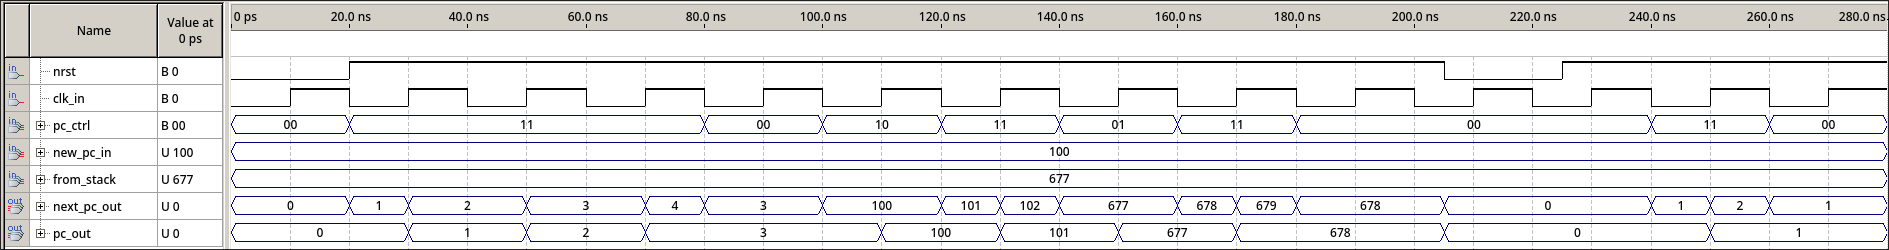
\includegraphics[width=\textwidth]{../../project/prog_cnt/prog_cnt_simulation.png}
  \fonte{Autoria própria (Quartus II).}
\end{figure}

\Needspace*{12\baselineskip}
{\scriptsize\setlength{\tabcolsep}{3pt}
\begin{longtable}{rccccccp{4.2cm}}
\caption{Casos de teste de \texttt{prog\_cnt.vwf}: visão geral.}
\label{tab:caso-prog-cnt}\\
\hline $t$ (ns) & \texttt{nrst} & \texttt{pc\_ctrl} & \texttt{new\_pc\_in} & \texttt{from\_stack} & \texttt{next\_pc\_out} & \texttt{pc\_out} & Observação \\ \hline \endfirsthead
\hline $t$ (ns) & \texttt{nrst} & \texttt{pc\_ctrl} & \texttt{new\_pc\_in} & \texttt{from\_stack} & \texttt{next\_pc\_out} & \texttt{pc\_out} & Observação \\ \hline \endhead
0--20 & 0 & 00 & 100 & 677 & 0 & 0 &  \\
20--40 & 1 & 11 & 100 & 677 & 2 & 1 & solta o reset; incrementa \\
40--60 & 1 & 11 & 100 & 677 & 3 & 2 & incrementa \\
60--80 & 1 & 11 & 100 & 677 & 4 & 3 & incrementa \\
80--100 & 1 & 00 & 100 & 677 & 3 & 3 & mantém (00) \\
100--120 & 1 & 10 & 100 & 677 & 100 & 100 & carrega new\_pc\_in = 100 \\
120--140 & 1 & 11 & 100 & 677 & 102 & 101 & incrementa \\
140--160 & 1 & 01 & 100 & 677 & 677 & 677 & carrega from\_stack = 677 \\
160--180 & 1 & 11 & 100 & 677 & 679 & 678 & incrementa \\
180--205 & 1 & 00 & 100 & 677 & 678 & 678 & mantém \\
205--225 & 0 & 00 & 100 & 677 & 0 & 0 & reset assíncrono \\
225--240 & 1 & 00 & 100 & 677 & 0 & 0 & solta o reset \\
240--260 & 1 & 11 & 100 & 677 & 2 & 1 & incrementa \\
260--280 & 1 & 00 & 100 & 677 & 1 & 1 & mantém \\
\hline
\end{longtable}}
\vspace{-0.9cm}
\fonte{Autoria própria. Saídas do fim de cada intervalo, conforme o modelo de referência e a simulação do Quartus II.}


\subsection{Análise dos resultados}

\begin{itemize}
  \item \textbf{Incremento}: com \texttt{pc\_ctrl = "11"} a partir de 20\,ns, \texttt{pc\_out} vai a 1, 2 e 3 nas bordas de 30, 50 e 70\,ns. Em cada ciclo \texttt{next\_pc\_out} já vale \texttt{pc\_out + 1} \textit{antes} da borda (o valor que será carregado).
  \item \textbf{Manutenção}: com \texttt{pc\_ctrl = "00"} (80--100\,ns), \texttt{next\_pc\_out} cai de 4 para 3 assim que \texttt{pc\_ctrl} muda, sem esperar o clock, e \texttt{pc\_out} permanece em 3.
  \item \textbf{Cargas}: com \texttt{pc\_ctrl = "10"}, \texttt{next\_pc\_out} vai a 100 (\texttt{new\_pc\_in}) imediatamente, e \texttt{pc\_out} só chega a 100 na borda de 110\,ns. Com \texttt{pc\_ctrl = "01"}, o mesmo ocorre com \texttt{from\_stack} (677). Em ambos os casos a outra entrada, que está com valor diferente, não tem efeito.
  \item \textbf{Reset assíncrono}: em 205\,ns, no meio do ciclo, \texttt{nrst} cai e \texttt{pc\_out} (678) vai a 0 na hora, e \texttt{next\_pc\_out} também, já que \texttt{pc\_ctrl = "00"} mantém o valor. Depois que o reset é solto, o incremento recomeça de 0.
\end{itemize}

Em \texttt{prog\_cnt\_incremento.vwf}, depois da carga de 2045, o contador passa por 2046 e 2047 e \textit{volta a 0} na borda seguinte, sem nenhuma lógica de comparação com 2047: a volta vem do tamanho de 11 bits do sinal. Em \texttt{prog\_cnt\_reset.vwf}, o reset ativo durante bordas com \texttt{pc\_ctrl = "11"} e depois \texttt{"10"} mantém o contador em 0, o que mostra que ele vence o incremento e a carga.
